%****************************************************************************%
%* Interface Presentation                                                   *%
%*                                                                          *%
%* Author(s):                                                               *%
%* - Abdelkader AMAR (Abdelkader.Amar@ens-lyon.fr)                          *%
%* - David LOUREIRO (David.Loureiro@ens-lyon.fr)                            *%
%*                                                                          *%
%* $LICENSE$                                                                *%
%****************************************************************************%
%* $Id: GUM_interface.tex,v 1.4 2007/11/29 16:03:21 dloureir Exp $
%* $Log: GUM_interface.tex,v $
%* Revision 1.4  2007/11/29 16:03:21  dloureir
%* typo corrections
%*
%* Revision 1.3  2007/11/08 16:28:53  dloureir
%* Adding some corrections and updates
%*
%* Revision 1.2  2007/11/08 11:31:14  dloureir
%* Correcting the headers
%*
%****************************************************************************%

\chapter{Interface presentation}

\grudu is composed of one principal frame shown in Figure \ref{fig:GRUDU_main}.
From this frame the user will be able to:
\begin{itemize}
  \item Log in \gfk
  \item Monitor \gfk and his/her reservations
  \item Have a terminal on the preferred access frontale, the different sites,
  and the main node of each of his/her reservations on \gfk
  \item Deploy images through KaDeploy on the appropriate nodes
  \item Exchange files between the locale machine and \gfk but also synchronize
  files between \gfk frontends.
  \item Log out
  \item Display the Help of \grudu
\end{itemize}

\begin{figure}[H]
\centering
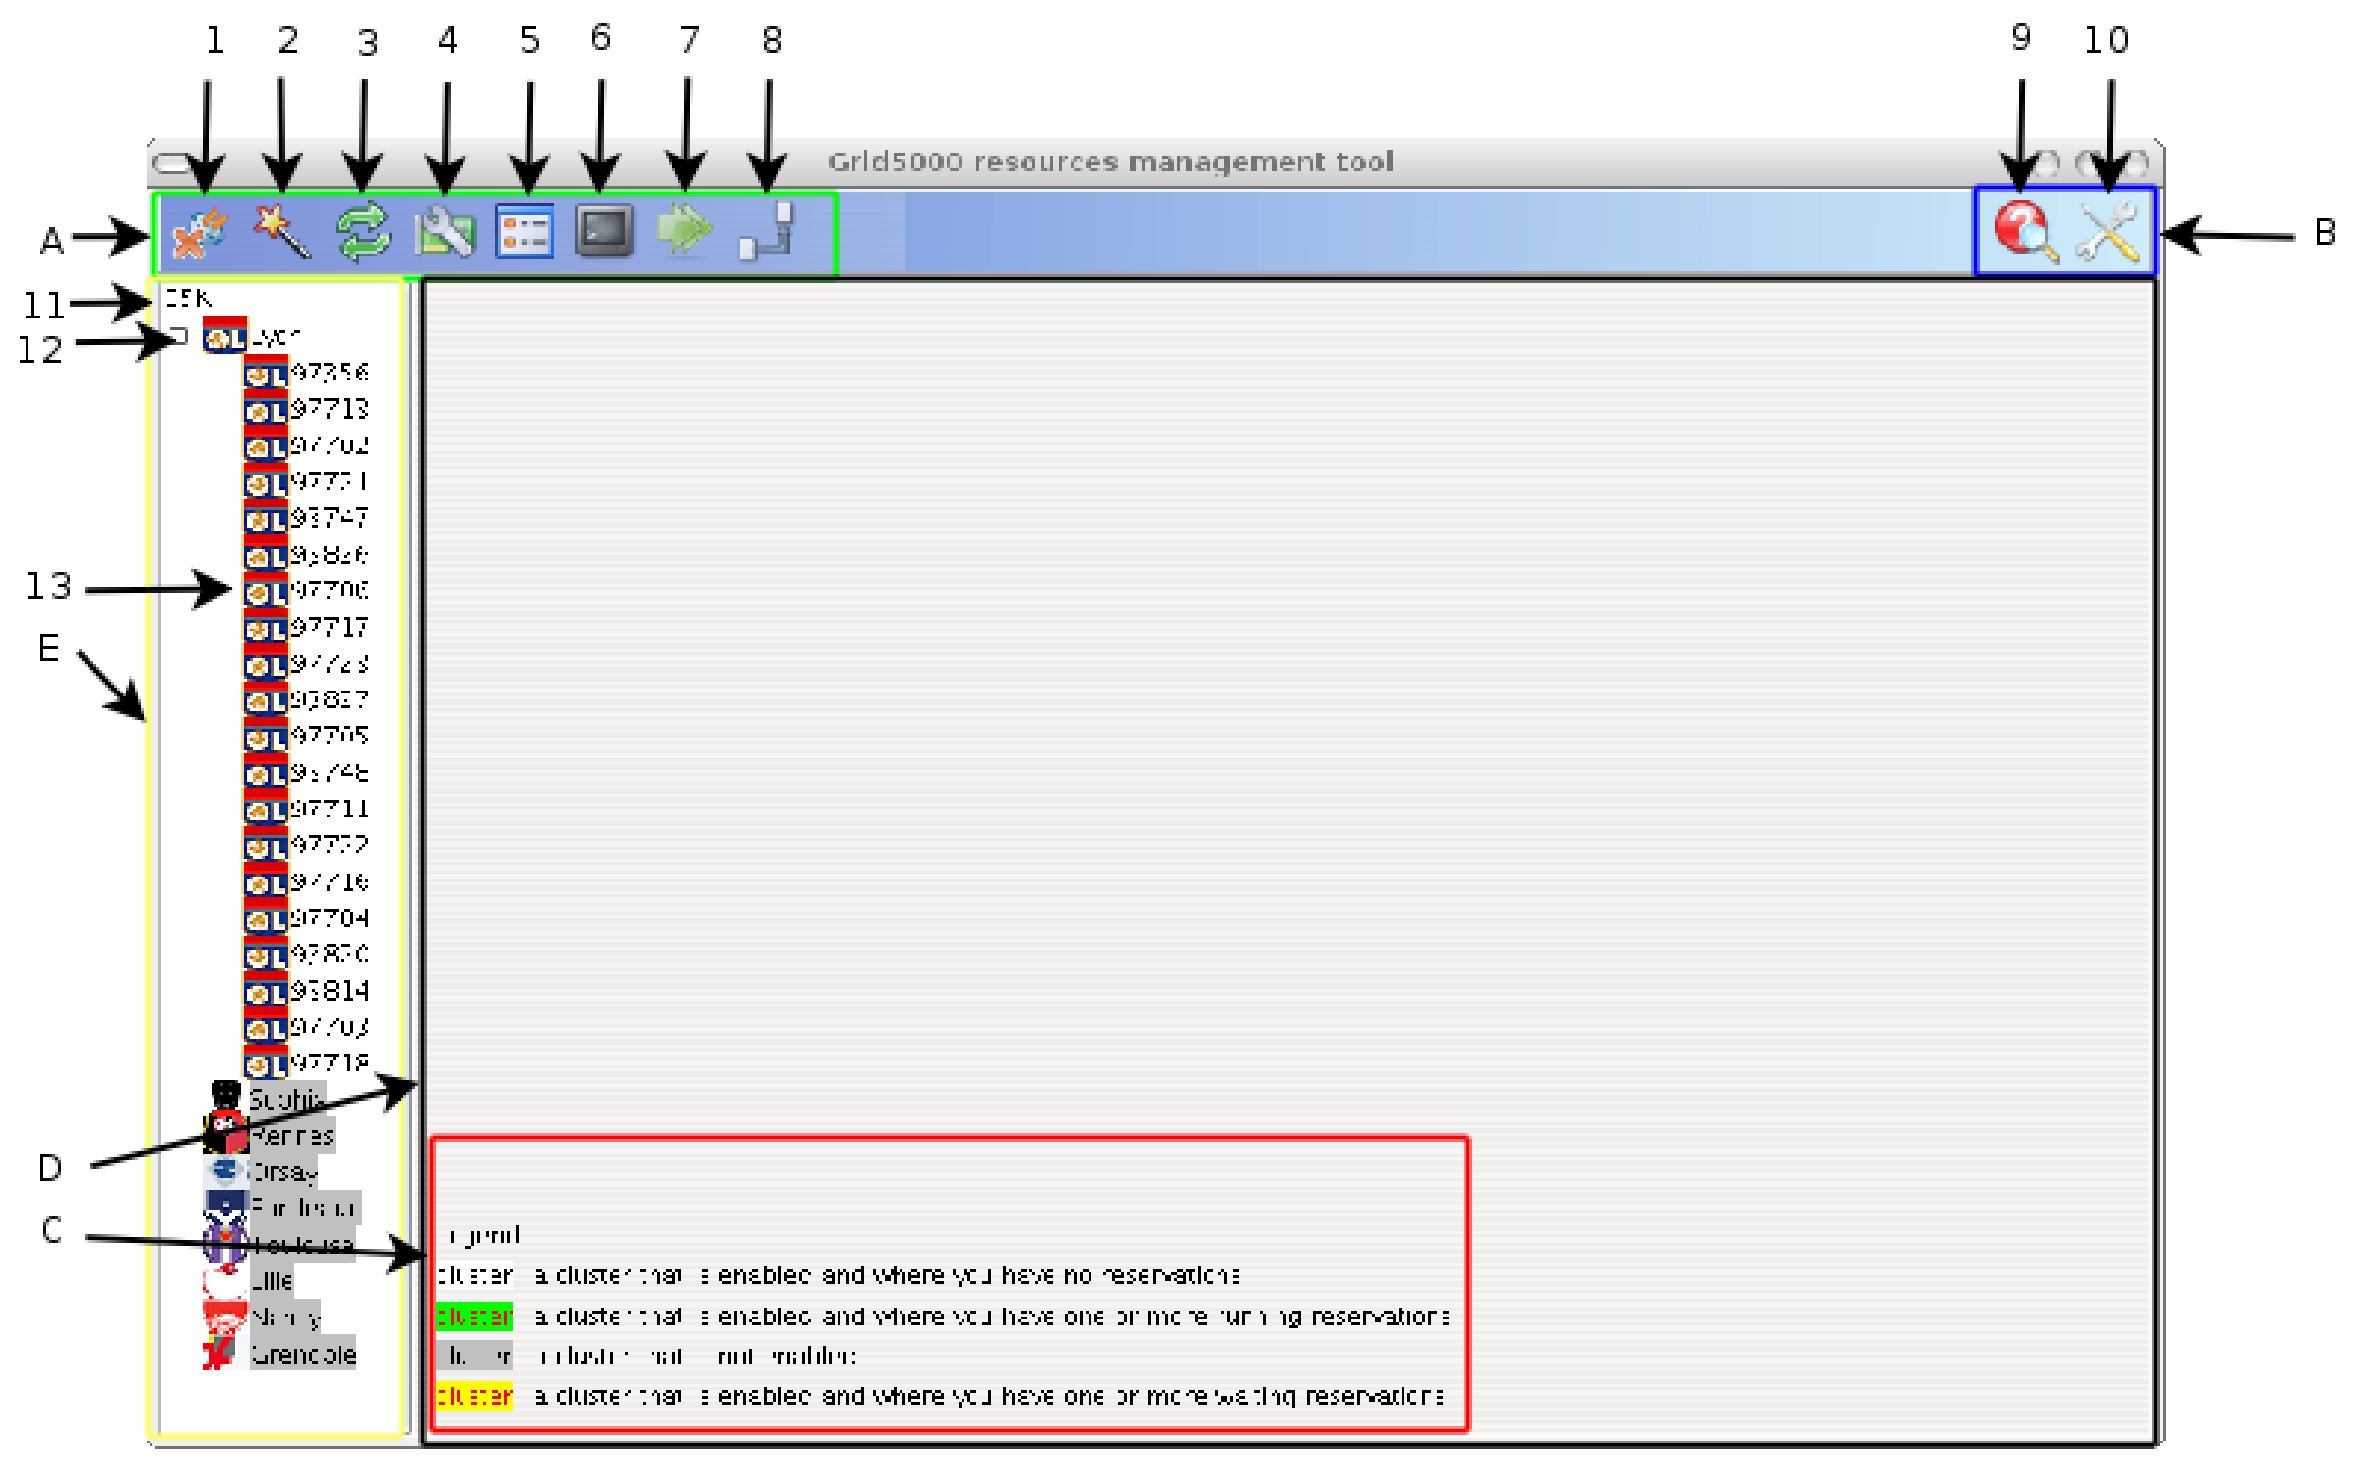
\includegraphics[width=\linewidth]{figures/GRUDU_interface_schema.eps}
\caption{Main interface of \grudu}
\label{fig:GRUDU_main}
\end{figure}

Legend of Figure \ref{fig:GRUDU_main}:
\begin{itemize}
  \item[A] Options toolbar (left-hand side).
  \begin{itemize}
    \item[1] Button used to log in \gfk (When connected to \gfk you will have a
    button to log out).
    \item[2] Button used to display the reservation frame.
    \item[3] Button used to update the \gfk tree of sites and jobs.
    \item[4] Button used to display the configuration frame.
    \item[5] Button used to display a summary of the information about \gfk and
    your reservations.
    \item[6] Button used to display a terminal on the preferred access point you
    have defined.
    \item[7] Button used to display the KaDeploy frame for the deployment of
    images with user-defined environments.
    \item[8] Button used to display the JFTP module for GRUDU. This module
    allows the user to transfert data between your locale machine and \gfk. You
    can also transfert data between the \gfk frontales.
  \end{itemize}
  \item[B] Options toolbar (right-hand side)
  \begin{itemize}
    \item[9] JavaHelp dedicated to the Help of GRUDU.
    \item[10] Application settings of GRUDU.
  \end{itemize}
  \item[C] Legend of the colors used for the sites, and jobs.
  \item[D] Main panel where information are displayed. Information about \gfk,
  the different sites and the jobs are displayed here.\item[]
  \item[E] \gfk sites and jobs.
  \begin{itemize}
    \item[11] Root node of the \gfk sites and jobs tree. This node
    allows you to display information about the grid. When right-clicking on this
    node, you can either update the \gfk view, open a shell on your preferred
    access point or delete all your reservations on \gfk.
    \item[12] Node corresponding to a site. Information about the site,
    i.e. the occupation of the nodes and the existing reservations on this
    site. When right-clicking on a site node, you can either delete the
    reservations you have on the site or open a shell on the site frontale.
    \item[13] Node corresponding to a job. Information on the job are displayed
    in the information panel. When right-clicking on that node, you will able to
    delete the corresponding reservation, update the site view or open a shell on
    the main node of the corresponding job.
  \end{itemize}  
\end{itemize}

A tip of the day frame is shown (if you want so) at GRUDU startup and presents
you some tips for the use of GRUDU. You can enable/disable the frame in the
application configuration frame (see \ref{chapter:application_settings}).

\begin{figure}[H]
\centering
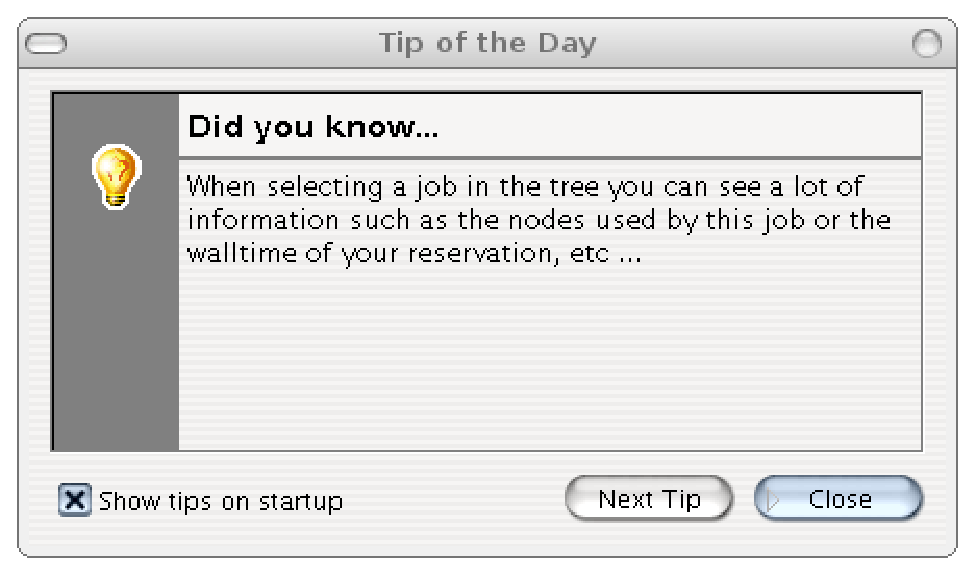
\includegraphics[width=0.6\linewidth]{figures/GRUDU_totd.eps}
\caption{Tip of the day for GRUDU}
\label{fig:GRUDU_totd}
\end{figure}

%******************************************%